\subsection{RQ3: How effective is context gathering for resolving kernel crashes?}%
\label{sec:rq3}

\begin{figure}[t]
    \centering
    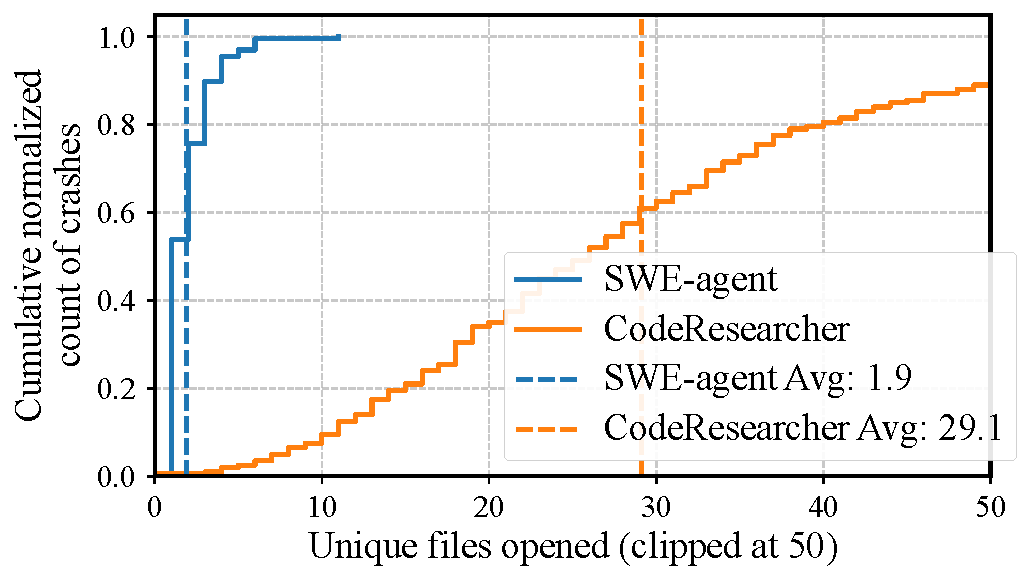
\includegraphics[width=0.45\linewidth,scale=0.4,keepaspectratio]{images/cdf_plot.pdf}
    \caption{Files explored for each crash (summed over 5 trajectories).}
    \label{fig:histogram}
\end{figure}
From Tables~\ref{tab:rq1-main} and \ref{tab:rq2-main}, \cresearcher{} (GPT-4o) significantly outperforms baselines that do not gather additional context but have high recall.
This shows that gathering global context (instead of just localizing the code to edit) can drastically improve kernel crash resolution.
Agentless, which does not gather any context, performs poorly, while
SWE-agent does gather context from the codebase, yet it performs much worse than \cresearcher{}.
Below, we investigate this further:

\noindent\textbf{1) Coverage of the context gathered:}
Figure~\ref{fig:histogram} shows the distribution of the number of unique files read across the $5$ trajectories by \cresearcher{} and SWE-Agent (GPT-4o, P@$5$, $15$ \maxcalls{}).
\cresearcher{} performs deep research over the codebase, reading $29.13$ unique files across $5$ top-level directories on average for each crash.
In stark contrast, SWE-agent reads only $1.91$ files on average for each crash.
When averaged by trajectory, \cresearcher{} explores $10$ unique files compared to only $1.33$ files explored by SWE-agent.

\noindent\textbf{2) Overlap with developer-referenced context:}
We use LLM-as-judge to determine the overlap of the context gathered by \cresearcher{}~(GPT-4o) and SWE-agent with the context mentioned by the developer in the fix commit message (details in Appendix~\ref{app:llm-as-judge}).
This context overlap is $54.18\%$ (over candidate patches) for SWE-agent compared to $63.7\%$ for \cresearcher{}, suggesting that \cresearcher{} does a much better job of identifying relevant context that the developer explicitly relied on when making the fix.

\noindent\textbf{3) Context quality when both edit all the ground-truth modified files:}
To isolate the impact of the gathered context,
we consider the subset of $90$ crashes, where both \cresearcher{} and SWE-agent (using the same GPT-4o model) edit \textit{all} the ground-truth files in \textit{at least one candidate patch} generated by each tool.
We can thus attribute their success (or failure) on this subset to the context gathered.
\cresearcher{} resolves $55/90 = 61.10\%$ of crashes in this subset, while SWE-agent resolves only $34/90 = 37.78\%$ (discounting crash-resolving patches from each tool that do not edit \textit{all} the ground-truth files).
\emph{Taken together, the three observations show that not only does \cresearcher{} gather more context than SWE-agent, it also gathers higher quality context.}
